% 
% Permission is granted to copy, distribute and/or modify this document
% under the terms of the GNU Free Documentation License, Version 1.2
% or any later version published by the Free Software Foundation;
% with no Invariant Sections, no Front-Cover Texts, and no Back-Cover
% Texts.  A copy of the license is included in the section entitled "GNU
% Free Documentation License".




%%%%%%%%%%%%%%%%%%%%%%%%%%%%%%%%%%%%%%%%%%%%%%%%%%%%%%%%%%%%%%%%%%%%%%%%%%%%%%%%%%%%%%%%%% 
\section{Use Cases Guide}


\subsection{UC1 : Creation and manipulation of an {\itshape IntegralUserDefined} variable}

This Use Case explicitates how to create and manipulate an $IntegralUserDefined$ variable which is a discrete variable with finite range and integer values.
\espace



\requirements{
  \begin{description}
  \item[$\bullet$] values of the range and associated probabilities : $range$ and $weights$
  \item[type:]  $range$ a python list of integers, $weights$ a list of reals, with unit sum or not
  \item[$\bullet$] or $sample$ a numerical sample of the discrete variable $X$
  \item[type:] a $NumericalSample$
  \end{description}
}
{
  \begin{description}
  \item[$\bullet$] a discrete variable with finite range and integer values : {\itshape myX}
  \item[type:] IntegralUserDefined
  \end{description}
}


\espace
Python  script for this Use Case :
\begin{lstlisting}

##############################################################################
# CASE 1 : Creation from the range values and the associated probabilities
##############################################################################

# Creation of the python list of the range (integers only)
# for example : 5, 7, 32
range = [5,7,32]

# Creation of the associated probabilities list
poidweightss = [0.1, 0.2, 0.3, 0.4]

# Creation of the IntegralUserDefined variable
myX = IntegralUserDefined(range, weights)

# Other signature
myX = IntegralUserDefined(UnsignedIntegerCollection(range), ...
     ... NumericalPoint(weights))


#########################################################
# CASE 2 : Creation form a numerical sample
#########################################################

# Creation of the IntegralUserDefined variable
myX = IntegralUserDefinedFactory.buildImplementation(sample)


########################################
# Manipulation of the IntegralUserDefined
########################################

# Get the range
print "range=", myd_Sc.getRange()

# Get thes weights 
print "weights=", myX.getWeights()

# Generate a realisation
print "realization=", myX.getRealization()

# Generate a numerical samplee
size = 10
print "numerical sample=", myX.getNumericalSample(size)

# Compute the probability of a particular state
print "weight of the value ", 5, "=", myX.computePDF(5)

# Compute the CDF of a particular state 
print "CDF at ", 5, "=", myX.computeCDF(5)
\end{lstlisting}




%%%%%%%%%%%%%%%%%%%%%%%%%%%%%%%%%%%%%%%%%%%%%%%%%%%%%%%%%%%%%%%%%%%%%%%%%%%%%%%%%
\subsection{UC2 : Creation and manipulation of an  {\itshape IntegralCompoundPoisson} variable}



This Use Case shows how to create and manipulate an {\itshape IntegralCompoundPoisson} variable, defined as :
\begin{equation}
Y = \left( \displaystyle \sum_{i=1}^{N}X_i \right)\fcar{N\geq 1}
\end{equation}

where $N$ is a Poisson distributed variable  parameterised by $\theta > 0$ and $(X_i)_i$  identically distributed random variables, with finite range and integer values. They are also mutually independent and also independent of $N$.

When a variable $Y$ of type $IntegralCompoundPoisson$ is created, all the values $p_k = \mathcal{P}(Y=k)$ are authomatically evaluated for $k \in [0, m-1]$ with $m = 2^{param}$. If the User asks for the evaluation of $p_n$ for $n \geq m$, then Open TURNS authomatically re-evaluates  all the values   $p_k$ for $k \in [0, N]$  with $N   = 2^{E[log_2 n]+1}$ (ie the first power of 2 which is strictly  $>n$).\\

The figures Fig. \ref{ICP_PDF} et Fig.\ref{ICP_CDF} draw the probability distribution and its cumulated probability distribution of an intergal compound distribution defined by : 
\begin{itemize}
  \item $(X_i)_i$ are distributed according to  the discrete distribution of range $[1, 2, 4, 7]$ associated to the respective probabilities $[0.1, 0.2, 0.3, 0.4]$,
  \item $N$ is a Poisson distribution which parameter is $\theta = 20$.
\end{itemize}


\begin{figure}[Hhbtp]
  \begin{minipage}{8cm}
    \begin{center}
      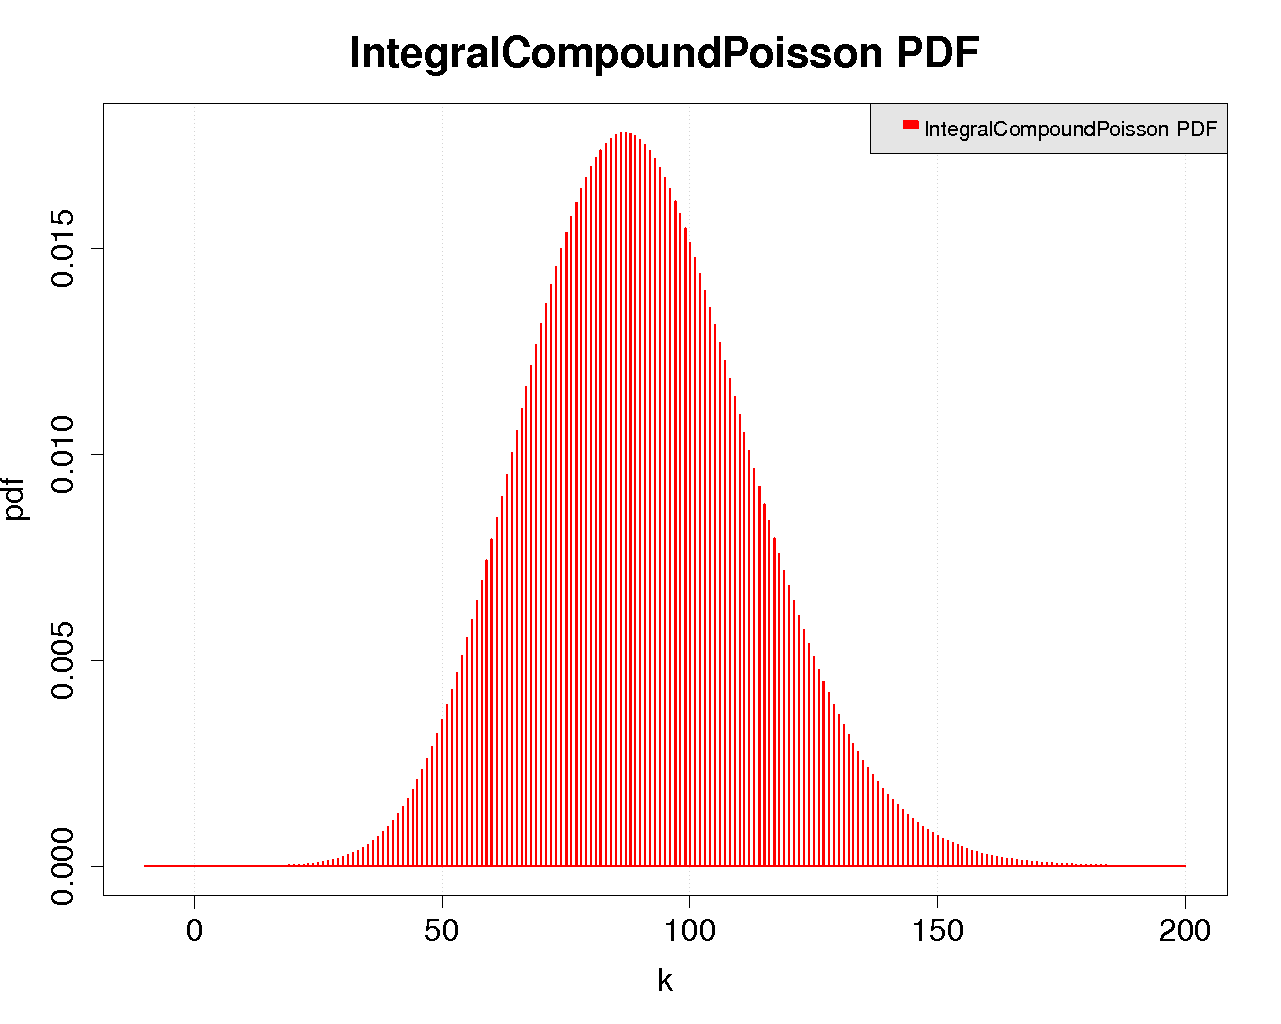
\includegraphics[width=8cm]{ICP_PDF.png} 
      \caption{Probability Distribution of an Integral Compound Poisson distribution.}
      \label{ICP_PDF}
    \end{center}
  \end{minipage}
  \hfill
  \begin{minipage}{8cm}
    \begin{center}
      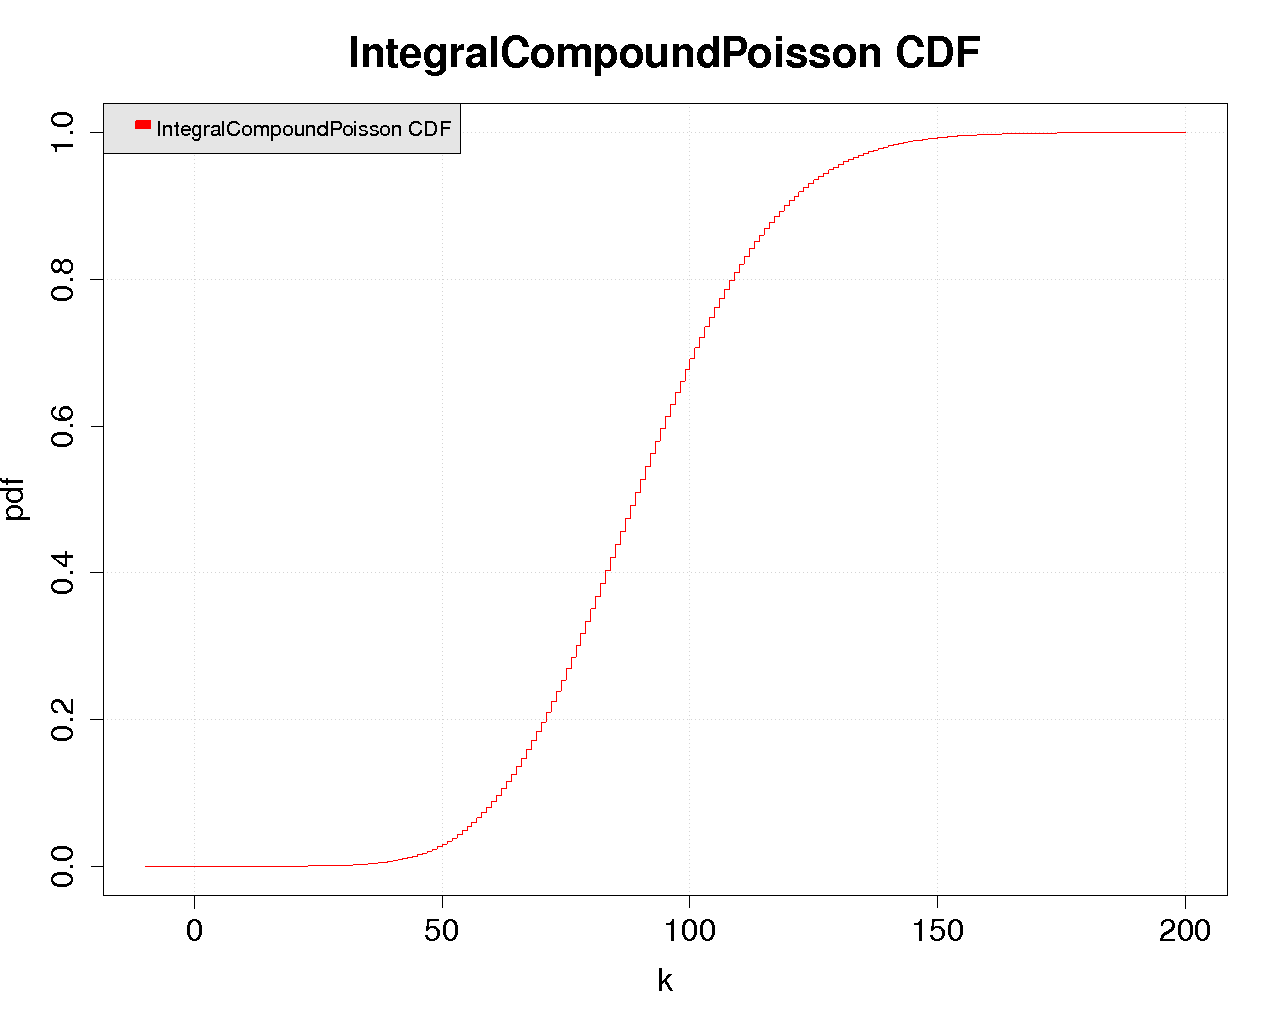
\includegraphics[width=8cm]{ICP_CDF.png} 
      \caption{Cumulated Probability Distribution of an Integral Compound Poisson distribution.}
      \label{ICP_CDF}
    \end{center}
  \end{minipage}
\end{figure}






\espace

\requirements{
 
  \begin{description}
  \item[$\bullet$] a discrete variable with finite range and integer values : {\itshape myX}
  \item[type:] a $IntegralUserDefined$
  \item[$\bullet$] the parameter of the Poisson distribution : {\itshape myTheta}
  \item[type:] a strictly positive real
  \end{description}
}
{
  \begin{description}
  \item[$\bullet$] a Integral Compound Poisson variable  : {\itshape myY}
  \item[type:] a $IntegralCompoundPoisson$
  \end{description}
}

\espace
Python  script for this UseCase :

\begin{lstlisting}
##########################################
# Creation  of the IntegralCompoundPoisson
##########################################

# Creation of the  IntegralCompoundPoisson variable
myY = IntegralCompoundPoisson(myX, myTheta)


###############################################
# Manipulation  of the  IntegralCompoundPoisson
###############################################

# Get the finite discrete distribution myX of type IntegralUserDefined
print "Inside IntegralUserDefined=", myYc.getAtomDistributionD()

# Get the Poisson parameter
print " Poisson parameter=", myY.getTheta()

# Get the param m
print "parameter m=", myY.getM()

# Get the param parameter
print "parameter param=", myY.getLog2cache()

# Generate a realisation of the distribution
print "realisation=", myY.getRealization()

# Compute the PDF at one particular point of the range
print "PDF at ", point, "=", myY.computePCDF(point5)

# Compute the CDF at one particular point of the range
print "CDF at ", point, "=", myY.computeCDF(point5)

# Compute the mean value
print "mean value=", myY.getMean()

# Compute the variance
print "variance=", myY.getCovariance()

# Compute the standard deviation
print "standard deviation=", myY.getStandardDeviation()

# Compute the quantile of order q
print "quantile order", q, "=", myY.computeQuantile(q)
\end{lstlisting}



%%%%%%%%%%%%%%%%%%%%%%%%%%%%%%%%%%%%%%%%%%%%%%%%%%%%%%%%%%%%%%
\subsection{Which python modules to import ?}

In order to use the functionalities described in this documentation, it is necessary to import  : 
\begin{itemize}
   \item the $oticp$ module which uses the $openturns$ module.
\end{itemize}

Python script for this use case :

\begin{lstlisting}
from openturns import *
from oticp import *
\end{lstlisting}
